\clearpage
\section{Blokové kódy}
\subsection{Stručně charakterizujte druhy blokových kódů.} \label{druhy}
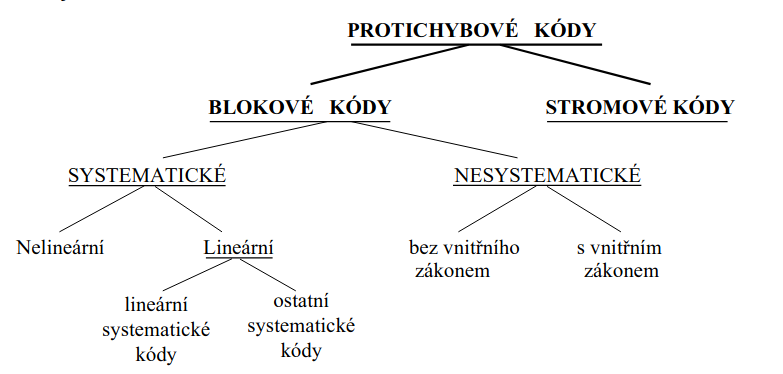
\includegraphics[width=16cm]{images/6_druhy.png}
\begin{itemize}
    \item systematické - rozložení informačních a zabezpečovacích bitů je stejné
    \begin{itemize}
        \item nelineární - nejsou lineární, vznikají např. kódovací tabulkou
        \item lineární - libovolnou kódovou kombinaci lze odvodit jako lineární kombinaci z ostatních kódových kombinací
        \begin{itemize}
            \item lineární systematické kódy - napřed se pošlou informační a na konci bloku jsou bity zabezpečovací
            \item ostatní lineární kódy - zabezpečovací bity jsou mezi informačními, na definovaných pozicích
        \end{itemize}
    \end{itemize}
    \item nesystematické - nerozlišují informační a zabezpečovací bity, zabezpečení spočívá v Hammingově vzdálenosti
    \begin{itemize}
        \item bez vnitřního zákona - správnost se ověřuje jen srovnáním s používanými bloky
        \item s vnitřním zákonem - mají jednoduché pravidlo určení správnosti přenosu (např. \uv{počet jedniček v bloku je 7})
    \end{itemize}
\end{itemize}

\subsection{Vysvětlete pojem lineární systematický blokový kód. Co znamená pojem lineární, co systematický a co blokový v problematice protichybových kódů?}
\begin{itemize}
    \item \textbf{Blokové kódy} - zabezpečovací proces je realizován pouze v rámci jediného bloku dat, který vznikl rozdělením datového toku
    \item \textbf{Systematické kódy} - můžeme zcela jednoznačně rozlišit v posloupnosti přenášených prvků informační prvky $k$ a zabezpečovací prvky $r$
    \item \textbf{Lineární kódy} - libovolnou kódovou kombinaci lze odvodit jako lineární kombinaci z ostatních kódových kombinací
\end{itemize}

\subsection{Podrobnější třídění blokových kódů a stručná charakteristika druhů blokových kódů.}
(viz. \ref{druhy})

\subsection{Co musí platit pro řádky vytvářecí matice lineárního blokového kódu. Jak vektory tvořící tyto řádky označujeme?}
\begin{itemize}
    \item Vytvářecí matice G má k řádků a n sloupců
    \item Řádky tvoří kódové kombinace, které jsou vzájemně lineárně nezávislé, tj. žádnou lineární operací mezi libovolnými řádky matice G nevznikne jiný řádek této matice
    \item Žádný z řádků matice nesmí obsahovat pouze nulové prvky
    \item Porovnáním řádků matice lze určit minimální Hammingovu vzdálenost $d_{min}$, která odpovídá minimální Hammingově vzdálenosti kódu $d_{min}$
    \item \textbf{Řádky} = generující vektory (báze vektorového prostoru)
    \item $G*H^{T}=0$
\end{itemize}

\subsection{Jaký je obecně vztah mezi vytvářecí a kontrolní maticí? Co tento vztah z hlediska
vektorových prostorů znamená?}
\begin{itemize}
    \item Vytvářecí matice $G=[I_{k\times k} C_{k\times r}]$, kde $I$ je jednotková matice, $C$ je zabezpečovací matice.
    \item Kontrolní matice $H=[C^T_{r\times k} I_{r\times r}]$ nebo ve tvaru $H^T=\left[ \begin{array}{cc}
        C_{k\times r} \\
        I_{r\times r}
    \end{array}\right]$
    \item $H$ generuje ortogonální vektorový prostor vůči $G$, platí $G\cdot H^T=0$
\end{itemize}

\subsection{Zapište maticově proces kódování a dekódování.}
\begin{itemize}
    \item kódování: $f=p\cdot G$, kde f je vysílaný blok
    \item dekódování: $j\cdot H^T=s$, kde j je přijatý blok a s je syndrom
\end{itemize}

\subsection{Vysvětlete princip funkce zapojení kodéru lineárního blokového kódu.}
$G=\left[\begin{array}{ccccccc}
    1 & 0 & 0 & 0 & 1 & 0 & 1 \\
    0 & 1 & 0 & 0 & 1 & 1 & 1 \\
    0 & 0 & 1 & 0 & 1 & 1 & 0 \\
    0 & 0 & 0 & 1 & 0 & 1 & 1
\end{array} \right]$, $r_1=p_1 \oplus p_2 \oplus p_3$ (první zabezpečovací bit je součet prvních 3 vstupů,
protože jedničky ve sloupci zabezpečovacího bitu $r_1$ jsou jedničky na 1., 2. a 3. řádku. Obdobně pak:
$r_2=p_2\oplus p_3 \oplus p_4$ a $r_3=p_1 \oplus p_2 \oplus p_4$\\
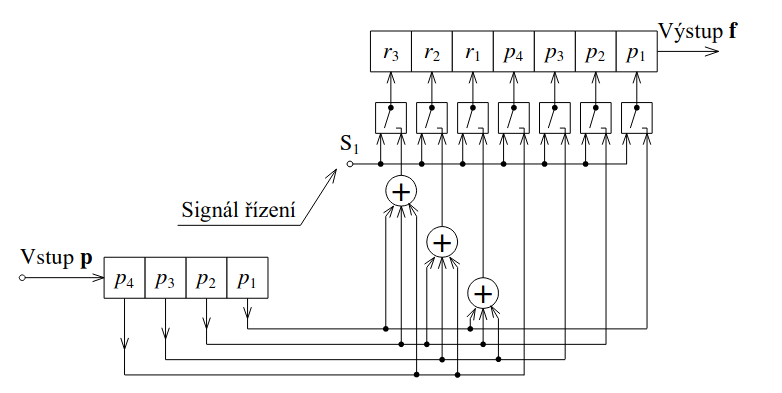
\includegraphics[width=16cm]{images/6_koder.png}

\subsection{Co je to syndrom. Vysvětlete vztah mezi syndromem, kontrolní maticí a chybovým
vektorem. Jak lze vytvořit tabulku syndromů?}
\begin{itemize}
    \item Syndrom je výsledek násobení přijatého vektoru s transponovanou kontrolní maticí. 
    Jedná se o kontrolu správnosti.
    \item Kontrolní matice slouží ke kontrole přijaté zprávy, generuje syndrom.
    \item Chybový vektor je binární vektor, označuje na kterých bitech došlo při přenosu k chybám. K jeho 
    nalezení slouží syndrom. Chybový vektor obsahuje jedničky na těch bitech, jejich pořadí odpovídá řádku transponované
    kontrolní matice, který je stejný jako syndrom. (např. třetí řádek kódu (7, 4) je [0 1 1], syndrom je stejný,
    chybový vektor je [0 0 1 0 0 0 0]
\end{itemize}

\subsection{Vysvětlete princip funkce zapojení dekodéru lineárního blokového kódu.}
Dekodér se skládá ze vstupní paměti, generátoru syndromu, generátoru chybového vektoru a korekce. Proběhne
maticové násobení, z něhož je nalezen syndrom. Ze syndromu nalezneme chybový vektor a ten přičteme 
k přijaté posloupnosti.

\subsection{Uveďte a vysvětlete jakým způsobem, jakou maticí jsou definovány základní Hammingovy kódy?}
\begin{itemize}
    \item Délka kódové kombinace: $n=2^m-1$
    \item r: $m$
    \item k: $2^m-1-m$
    \item $m \geq 3$
    \item Kontrolní matice je počítána binárním zápisem čísel do sloupců. Např. kód (7, 4):\\
    $H=\left[\begin{array}{ccccccc}
        0 & 0 & 0 & 1 & 1 & 1 & 1 \\
        0 & 1 & 1 & 0 & 0 & 1 & 1 \\
        1 & 0 & 1 & 0 & 1 & 0 & 1
    \end{array}
    \right]$
    \item Transponovaná matice $H^T$ vznikne jednoduchým transponováním.
    \item Zabezpečovací bity: $r_1 = 3 \oplus 5 \oplus7$, $r_2 = 3 \oplus 6 \oplus 7$,
    $r_3 = 5 \oplus 6 \oplus 7$ (od druhé jedničky na každém řádku kontrolní matice, číslování řádků odspodu)
\end{itemize}
